\documentclass[12pt,oneside]{report}
\usepackage[a4paper]{geometry}
%\usepackage{showkeys}
\usepackage{listings}
\lstset{
language=C,
basicstyle=\tiny\ttfamily}

\usepackage{draftcopy}
\draftcopyName{Joao Paulo}{180}
\usepackage{joaopaulo}
\title{Apostila de Automação Industrial}
\begin{document}

\maketitle
\tableofcontents
\chapter{Sistemas de automação}
%!TEX root = apostila.tex
% \section{Definição}
\label{chap:automacao}
A palavra automação vem do latim \emph{automatus} -- mover por si mesmo. Logo a automação de uma tarefa consiste em fazer com que tal tarefa seja realizada sem envolver trabalho humano. Isto pode ser por diversos motivos: seja por que é uma tarefa perigosa e portanto queremos aumentar a segurança das pessoas, seja para fazer a tarefa de forma mais rápida, seja para melhorar a qualidade do produto final ou seja porque simplesmente o custo do trabalho humano é muito elevado. Logo, podemos definir automação da seguinte forma:
\begin{quote}
  Automação é a substituição do trabalho humano por sistemas autônomos visando melhorar segurança, qualidade, produção e/ou custos.
\end{quote}

Neste contexto, automação industrial é nada mais que a automação de um sistema industrial, ou de um sistema de manufatura. Embora manufatura venha de \emph{fazer com as mãos}, desde a revolução industrial que usamos esta palavra significando simplesmente a fabricação de algum produto. Juntando então o conceito de automação, têm-se:
\begin{quote}
  A automação industrial consiste em implementar os processos necessários para a manufatura de algum produto com o mínimo de esforço humano, físico ou mental, visando melhor segurança, qualidade, produção e/ou custo.
\end{quote}

Com base nesta definição, qualquer sistema que realize a manufatura de algum produto automaticamente e sem usar esforço humano é um sistema automatizado. Logo, uma máquina por mais complexa que seja mas que funcione a manivela, tal como uma calculadora mecânica, não se classifica como automação. Da mesma forma uma máquina que não exija esforço físico mas requeira atenção constante, tal como um carro ou mesmo uma batedeira, também não é automatizada; neste último caso usa-se o termo mecanizada.

Do ponto de vista econômico, a manufatura é a transformação de materiais (matéria prima) em itens de maior valor (produto). Isto é conseguido por uma determinada sequência de processos químicos e físicos. De forma mais sucinta:
\begin{quote}
	Manufatura é a transformação de matéria prima em produtos pela aplicação de um ou mais processos.
\end{quote}

Ou seja, na automação industrial estamos interessados em estudar métodos e ferramentas que permitam deixar os processos de manufatura os mais independentes possível da interferência humana. 

\section{Classificação}

O próprio avanço dos sistemas de automação permite com que se tenham equipamentos cada vez mais versáteis, que não sejam feitos para a fabricação de um único produto. Esta possibilidade de equipamentos versáteis levam a, grosso modo, 3 tipos de automação, tal qual mostra a figura \ref{fig:tipos_automacao}: fixa, flexível e programável. Tipicamente são fatores econômicos que levam a escolha de um destes tipos.

\begin{figure}[hbt]
	\begin{center}
    \includegraphics[width=0.8\textwidth  ]{figuras/fixaflexprog}
%		\includegraphics[width=0.6\textwidth]{tipos_automacao}
	% \tikzstyle{area}=[draw,rectangle,rounded corners,text centered,text width=2.2cm,minimum height=1.2cm]
	% \begin{tikzpicture}
	% 	\draw[very thick, ->, >=stealth'](0,0)--(5.5,0);
	% 	\draw(5.5,0)node[below left]{Diversidade};
	% 	\draw[very thick, ->, >=stealth'](0,0)--(0,3.3);
	% 	\draw(0,3.3)node[above left, rotate=90]{Quantidade};
	% 	\draw(1.25,2.5)node[area]{Fixa} (2.5,1.55)node[area]{Flexível} (4,0.6)node[area]{Programável};
	% \end{tikzpicture}
	\end{center}
	\caption{Tipos de automação industrial quanto a quantidade e diversidade de produtos.}
	\label{fig:tipos_automacao}
\end{figure}

A automação fixa é aplicada à produção de um único produto (ou com mínimas variações), em grandes quantidades: refinaria de petróleo, parafuso, tampas de garrafa, clipes de papel, elos de corrente, biscoito, cerveja, etc. Ela utiliza equipamentos feitos sob medida para cada processo, que portanto tem alto custo inicial mas grande produtividade.

A automação flexível é aplicada à produção de produtos parecidos, em que pequenas modificações permitem a alteração do produto, como por exemplo mudança de um perfil a ser prensado ou extrudado ou a mudança das quantidades do mesmo conjunto de matérias primas (mudança de receita). Tipicamente é feita a chamada fabricação em lotes, onde entre um lote e outro se alteram as peças e/ou as sequências a serem seguidas de forma automática para ter o menor tempo parado possível. Exemplos são livros, circuitos integrados, potes de plástico, panelas, entre outros.

A automação programável é para produção de produtos diferentes mas cujo volume de produção não justifica um processo único. Ela usa máquinas de propósito geral, tais como robôs, ferramentas de controle numérico e impressoras 3d, onde a definição do processo é quase toda feita por \emph{software}, de modo que o custo do maquinário é diluído em diversos produtos.

Estes três tipos não são precisamente definidos, e fica difícil, muitas vezes, determinar que ponto separa uma automação deixa fixa de uma flexível, ou flexível de programável. Por exemplo, uma fábrica de tampas de garrafa PET, que fabrica tampas vermelhas e verdes, em lotes, deixa de ser fixa por conta da mudança da cor?

Mas quanto mais flexível for o sistema de automação, mas necessitado ele é de sistemas de informática e de equipamentos de uso geral controláveis. De modo geral, a automação fixa pode ser realizada a nível de Indústria

A tendência é cada vez mais ter a automação flexível e programável aumentando a capacidade de produção, de modo que a flexível vai ocupando nichos da fixa e a programável da flexível. Apesar disso, em vários casos é difícil imaginar alguns produtos deixando de utilizar a automação fixa.

\section{Pirâmide de automação}

A automação em larga escala de uma grande indústria envolve muito mais que a mera manufatura e inclui problemas de abastecimento, armazenagem, análise de mercado, exigências ambientais, entre várias outras coisas. Uma forma de se separar os diferentes problemas da automação é através da chamada Pirâmide de Automação, mostrada na figura \ref{fig:piramide}.

\begin{figure}[htb]
	\begin{center}
\begin{tikzpicture}[y=0.80pt, x=0.8pt,xscale=0.4,yscale=-0.4, inner sep=0pt, outer sep=0pt]
    \path[fill=black] (530,582.41803) node[above right] (text3018)
      {Instrumentação};
    \path[fill=black] (530,511.83002) node[above right] (text3022) {Controle};
    \path[fill=black] (530,441.0715) node[above right] (text3794)
      {Supervisão};
    \path[fill=black] (530,370.13507) node[above right] (text3798) {Gerência
      de manufatura};
    \path[fill=black] (530,299.51303) node[above right] (text3804)
      {Planejamento estratégico};
      \path[cm={{1.01932,0.0,0.0,1.01932,(-6.1462,-4.25386)}},draw=black,fill=c00ffff,miter
        limit=4.00,line width=2pt] (320.0000,252.3622) -- (423.9230,432.3622) --
        (527.8461,612.3622) -- (320.0000,612.3622) -- (112.1539,612.3622) --
        (216.0770,432.3622) -- cycle;
      \path[cm={{0.80176,0.0,0.0,0.79778,(63.47204,51.63306)}},draw=black,fill=c00ff00,miter
        limit=4.00,line width=2pt] (320.0000,252.3622) -- (423.9230,432.3622) --
        (527.8461,612.3622) -- (320.0000,612.3622) -- (112.1539,612.3622) --
        (216.0770,432.3622) -- cycle;
      \path[cm={{0.60132,0.0,0.0,0.59833,(127.61319,101.96534)}},draw=black,fill=cffff00,miter
        limit=4.00,line width=2pt] (320.0000,252.3622) -- (423.9230,432.3622) --
        (527.8461,612.3622) -- (320.0000,612.3622) -- (112.1539,612.3622) --
        (216.0770,432.3622) -- cycle;
      \path[cm={{0.40088,0.0,0.0,0.39889,(191.75434,152.29762)}},draw=black,fill=cff6600,miter
        limit=4.00,line width=2pt] (320.0000,252.3622) -- (423.9230,432.3622) --
        (527.8461,612.3622) -- (320.0000,612.3622) -- (112.1539,612.3622) --
        (216.0770,432.3622) -- cycle;
      \path[cm={{0.20044,0.0,0.0,0.19944,(255.8955,202.62989)}},draw=black,fill=cff5555,miter
        limit=4.00,line width=2pt] (320.0000,252.3622) -- (423.9230,432.3622) --
        (527.8461,612.3622) -- (320.0000,612.3622) -- (112.1539,612.3622) --
        (216.0770,432.3622) -- cycle;
    \begin{scope}[shift={(3.29592,0)}]
      \path[fill=black] (309.04346,582.41803) node[above right] (text3824) {0};
      \path[fill=black] (310.00049,511.8302) node[above right] (text3828) {1};
      \path[fill=black] (309.28271,441.0715) node[above right] (text3832) {2};
      \path[fill=black] (309.00244,370.13507) node[above right] (text3836) {3};
      \path[fill=black] (309.45361,299.51303) node[above right] (text3840) {4};
    \end{scope}
    \path[fill=black] (79.834969,582.41803) node[above left] (text3858) {Sensores
      eatuadores};
    \path[fill=black] (79.875984,511.8302) node[above left] (text3862) {CLP, SDCD,
      CNC};
    \path[fill=black] (81.256844,441.0715) node[above left] (text3866) {SCADA,
      HMI};
    \path[fill=black] (80.245125,370.13507) node[above left] (text3870) {PIMS, MES,
      LIMS, WMS};
    \path[fill=black] (79.999031,299.51303) node[above left] (text3874) {ERP};

\end{tikzpicture}
	\end{center}
	\caption{Pirâmide de automação.}
	\label{fig:piramide}
\end{figure}

Note que esta não é a única representação da pirâmide: umas começam pelo 1, outras tem apenas 4 camadas, e assim por diante, logo mais importante que o número de cada camada é o que tais camadas significam.

\begin{description}
	\item[Nível 0: Instrumentação] Camada onde se encontram instrumentos, sensores, motores,
máquinas, etc. Consistem nos equipamentos do chamado ``\emph{chão de fábrica}''.
\item[Nível 1: Controle] Controle automático da planta -- onde se localizam os Controladores
Lógico-Programáveis (CLP), os Sistemas Digitais de Controle Distribuído (SDCD), os Controles Numéricos Computadorizados (CNC) e/ou computadores de controle.
\item[Nível 2: Supervisão] Supervisão e controle do processo através de Interfaces Homem-Má
quina (IHMs) ou SCADA (\emph{Supervisory Control And Data Acquisition}).
\item[Nível 3: Gerenciamento da Manufatura] Gestão dos recursos da planta e controle da produção.  Sistemas PIMS
(\emph{Process Information Management System}) e MES (\emph{Manufacturing Execution Systems}).
\item[Nível 4: Planejamento Estratégico] Gestão dos recursos e produção da empresa como um todo. ERP –
\emph{Enterprise Resources Planning}.
\end{description}

A figura \ref{fig:automacao} mostra um diagrama em blocos de um processo automatizado, contendo os blocos representativos dos níveis 0 a 3 da pirâmide de automação. A instrumentação consiste de sensores e atuadores. As variáveis medidas pelos sensores são denominadas de variáveis controladas, enquanto que os valores de comando dos atuadores são chamados de variáveis manipuladas. Como tais atuadores irão operar é definido pelo controle (nível 1), em função de parâmetros definidos pelo supervisório, (nível 2). Este também monitora estas informações e as repassa ao sistema de gerenciamento no nível 3, que aglutina dados de diversos processos para a tomada de decisões de mais alto nível.
\begin{figure}[htb]
	\begin{center}
    \includegraphics[width=0.7\textwidth]{figuras/automacao}
	\end{center}
	\caption{Diagrama em blocos da automação de um processo.}
	\label{fig:automacao}
\end{figure}

Este texto faz um estudo da automação industrial de modo \emph{bottom-up}: começando do nível 0 até o nível 3. O nível 4 é mais importante para um estudo de engenharia de processo ou de produção e portanto não será abordado.

%!TEX root = principal.tex
\chapter{Gerenciamento da manufatura: PIMS e MES}

 PIMS -- \emph{Process Information Management System} e MES -- \emph{Manufacturing Execution System} são sistemas da camada 3 da pirâmide de automação, responsáveis pelo armazenamento e tratamento de dados do nível 2, concentrando os dados de diversos processos separados em um único ponto. São os chamados \emph{middleware}, pois ficam a meio caminho entre os sistemas de gerenciamento de empresa e os supervisórios, às vezes combinando funções de um ou de outro.

 De forma geral, no terceiro nível da pirâmide a preocupação é em consolidar os dados brutos do processo (\emph{data}), para com eles gerar informações  (\emph{information}) e conhecimento (\emph{knowledge}) sobre o processo, aumentando o valor destes valores, como mostra a figura \ref{fig:PIMS_conhecimento1}. Os dados são obtidos ou do controlador ou do supervisório de um determinado processo. A relação entre dados ou a variação destes dados no tempo geram informação sobre a planta. A relação entre informações ou a variação de informações no tempo geram conhecimento.
\begin{figure}[htb]
	\begin{center}
	%	\includegraphics[angle=-90,width=0.8\textwidth]{PIMS_conhecimento1}
		\begin{tikzpicture}[scale=1.5]
		\draw[very thick, ->, >=stealth'](0,0)--(5.5,0);
		\draw(5.5,0)node[below left]{Quantidade de dados};
		\draw[very thick, ->, >=stealth'](0,0)--(0,3.3);
		\draw(0,3.3)node[above left, rotate=90]{Valor};
		\draw[very thick] plot[smooth, tension=1.0] coordinates{(0.2,3.3) (2,1) (5.5,0.3)};
		\draw(0.3,3.)node[right]{Conhecimento} (1.3,1.4)node[above right]{Informação} (4.3,0.4)node[above]{Dados brutos};
	\end{tikzpicture}

	\end{center}
	\caption{Relação entre dados, informações e conhecimentos.}
	\label{fig:PIMS_conhecimento1}
\end{figure}

Um exemplo desta relação é mostrado na figura \ref{fig:PIMS_conhecimento2}. Nesta figura, a partir dos dados de temperatura e vazão de um fluido é gerada a informação do calor removido em determinado trocador de calor. A comparação dos calores removidos de diversos trocadores gera o conhecimento de qual trocador é mais eficiente.

\begin{figure}[htb]
	\begin{center}
		
\includegraphics[angle=-90,width=0.8\textwidth]{PIMS_conhecimento2}
	\end{center}
	\caption{Exemplo da transformação de dados para informação e de informação para conhecimento.}
	\label{fig:PIMS_conhecimento2}
\end{figure}

\section{PIMS}
	Para a finalidade de gerar informação e conhecimento, o ponto de partida é obter os dados brutos. Esta é a tarefa principal do PIMS: adquirir, armazenar e apresentar diversos dados de uma planta. O PIMS foi criado e ainda é principalmente usado para processos contínuos, tais como uma refinaria ou siderúrgica, e portanto tem um enfoque muito grande em variáveis analógicas e na relação delas com o tempo.

	Do ponto de vista do PIMS podemos esquematizar os sistemas de uma fábrica como mostra a figura \ref{fig:PIMS}, onde se vê que o PIMS tem 4 partes principais: um
	\begin{description}
		\item[historiador de processos] que se comunica com vários sistemas do nível 1 (CLP, CNC) ou 2 (supervisório) ou ainda de outros sistemas nível 3, tais como um LIMS -- \emph{Laboratory Information Management System} ou MES para obter dados brutos dos diversos processos e acumula-os num
		\item[banco de dados temporal], que armazena os dados indexando-os pelo tempo. Uma
		\item[interface gráfica] faz a recuperação e visualização destes dados, que ainda podem ir para
		\item[aplicações clientes] com variadas funções, desde análise dos dados a interface com outros sistemas.
	\end{description}
	\begin{figure}[hbt]
		\begin{center}
			\includegraphics[angle=-90,width=0.8\textwidth]{PIMS}
		\end{center}
		\caption{Sistema PIMS -- REFAZER.}
		\label{fig:PIMS}
	\end{figure}

\subsection{Historiador de Processos}
O historiador do processo é necessário pelas seguintes funcionalidades:
\begin{description}
 	\item[Registro Histórico] para análise de incidentes, controle de qualidade, métricas de performance, entre outros.
 	\item[Adequação a normas] como por exemplo para controle ambiental.
 	\item[Monitoração de equipamentos] para ontrole de vida útil e apoio à manutenção.
 	\item[Análise de processo], facilitando a visualização de dados e detecção de correlações.
 \end{description}  			

Para tanto o historiador se comunica com sistemas do nível 2 (SCADA) e 1 (CLP) para armazenar os dados do processo. Estes dados são principalmente os valores das variáveis do processo, sejam discretos ou contínuos, mas também abarcam outras informações, tais como a ocorrência de alarmes, a marcação de que operador está presente, o período que um equipamento está ligado, entre outros. Cada uma desta isformações é identificada por um marcador único - a chamada \emph{tag}, ao qual também está associado o endereço lógico de onde se obtém tal informação e o tempo em que tal dado foi gerado (\emph{time stamp}). Em alguns casos se associa também uma métrica da qualidade do dado, referente a confiabilidade daquele dado, tal como se o instrumento de medida está calibrado ou não.

Estas informações podem ser obtidas tanto de sistemas SCADA ou de CLPs. Algumas vantagens de pegar informação dos sistemas nível 2 são que: 
\begin{itemize}
	\item o SCADA já converteu os dados para unidades de engenharia enquanto que em alguns CLPs os dados estão em valor bruto (de 0 a 4095);
	\item muitas variáveis são definidas apenas no sistema SCADA, não existindo nos CLPs, tais como o motivo de alarmes ou qual operador está monitorando a operação;
	\item  interface com os sistemas SCADA costuma ser padrão, o que facilita a comunicação e interoperação.
\end{itemize}

Vantagens de obter as informações do CLP são:
\begin{itemize}
	\item busca dos eventos com menor atraso temporal;
	\item pode-se coletar os dados em um ponto único, se todas as redes de CLPs estiverem interligadas;
	\item CLPs são mais confiáveis e apresentam menor suscetibilidade a falhas que os sistemas SCADA.
\end{itemize}

\subsection{Banco de Dados Temporal}
A maioria das análises realizadas nos dados de um sistema PIMS são em função do tempo, logo é comum ele usar um banco de dados que indexa a informação pelo tempo. Basicamente é uma tabela, relacionando \emph{time stamp}, \emph{tag}, tipo de dado (analógico, booleano, texto), valor e qualidade (se houver).

Um problema do uso deste tipo de banco de dados, ao invés dos chamados bancos de dados relacionais, que são bem mais comuns, é que a busca por informação pode ter uma baixa performance quando a quantidade de dados aumenta muito. Esta é a principal razão para que estes sistemas façam uma compressão de dados, que basicamente se resume a não armazenar dados que não tragam muita informação nova. A figura \ref{fig:reconstrucaoDados} mostra a idéia por trás da compressão de dados.

\begin{figure}[hbt]
	\begin{center}
		\includegraphics[width=0.8\textwidth]{figuras/reconstrucaoDados}
	\end{center}
	\caption{Processo de amostragem, compressão e reconstrução dos dados.} %%TODO:refazer
	\label{fig:reconstrucaoDados}
\end{figure}

Algoritmos comuns para a compressão de dados no PIMS são \emph{banda morta}, onde os dados são apenas armazenados se variarem mais do que um mínimo especificado; o \emph{SDCA -- Swinging Doors Compression Algorithm}, onde para cada valor recebido é definida uma reta entre ele e o último valor armazenado, descartando valores que possam ser definidos por esta reta e mais um erro; e o \emph{boxcar/backslope}, que usa a banda morta e mais uma reta definida pelo último valor armazenado. %%Pequeno. Pode ser expandido

\subsection{Interface Gráfica}
A interface gráfica de um sistema PIMS é, em muitos aspectos, muito parecida com a de um sistema SCADA, contendo representações pictóricas do processo (sinóticos) com os valores de várias variáveis e gráficos de tendência. Tais elementos são melhor vistos no contexto de um sistema SCADA.

\section{MES}
Assim como o PIMS, um sistema MES também adquire dados do processo com o objetivo de apresentar uma visão geral do processo. Porém o MES tem uma função mais ativa que o PIMS, que é focado mais no armazenamento dos dados. Outra diferença importante é que os MES são usados principalmente em processos discretos, muitas vezes em sistemas de automação flexível ou programada, e tem que lidar com o sequenciamento dos processos, o que ocorre menos em sistemas contínuos.

Os sistemas MES agregam diversas funções de sistemas anteriores mais simples e específicos e são definidos por terem 11 funções:
\begin{description}
	\item[Gerenciamento das definições de produto.] Tudo o que é necessário para a fabricação do produto. Isto inclue armazenamento, lista de materiais e insumos, set-points do processo e receitas.

	Por receita, entenda-se uma variação do processo para, na mesma máquina, produzir produtos diferentes ou variações dele. Por exemplo, num processo de pintura a receita diria quais as tintas usadas, em que sequência, em que volume e em que velocidade de aplicação. É muito importante na automação flexível e programável.

	\item[Gerenciamento de insumos.] Permite preparar e executar ordens de produção com garantia de disponibilidade dos insumos.
	\item[Agendamento de produção.] Permite determinar a ordem que a produção será feita, para alcançar os requerimentos de produção definidos pela ERP (camada 4 da pirâmide) utilizando otimamente os recursos.

	Tipicamente inclui ferramentas de simulação, que permitem comparar diversas opções de ordens e estimar efeitos quando de mudanças imprevistas na sequência de produção (tipicamente por conta de uma parada não programada).

	\item[Envio de ordens de produção.] Em função do agendamento feito, o MES cuida de enviar as ordens de produção para os diversos postos da planta.
	\item[Acompanhamento da execução de ordens de produção.] Comunicação com sistemas níveis 1 e 2 para garantir a execução das ordens. Inclui também o registro de paradas.

	O registro de paradas é feito automaticamente quando o equipamento para, seja por alguma condição espúria detectada no nível 1 ou por ação do operador no nível 2. Em ambos os casos fica registrado uma parada em aberto, que só finaliza quando o operador complementar certas informações que auxiliam no diagnóstico da parada e o equipamento voltar a funcionar.

	\item[Coleção dos dados de produção.] Equivalente ao historiador de processo do PIMS.
	\item[Análise da performance da produção.] Cálculo dos chamados índices de produção -- \emph{KPI, Key Performance Indicators}. É a geração de informação útil a partir dos dados da produção.

	Como exmplo de um KPI, temos o OEE -- \emph{Overall Equipment Effectiveness} -- que aponta a efetividade de um determinado equipamento ou célula de produção. Este índice é dado por:

\begin{equation}
	\text{OEE} = \text{disponibilidade}\times\text{performance}\times\text{qualidade,}
\end{equation}
onde por disponibilidade entende-se a razão entre o quanto de tempo o equipamento funcionou e o quanto de tempo ele deveria ter funcionado, ou seja, descontando-se as paradas não programadas; performance é a razão entre a produção do equipamento enquanto funcionava e a capacidade de produção de que o equipamento é capaz, ou seja, descontando a ociosidade do equipamento; e qualidade é o valor do que o equipamento produziu em relação ao valor se não tivesse havido nenhum descarte ou geração de produtos de menor valor.

	\item[Rastreamento da produção.] Permite levantar que produto ou lote foi feito quando e em qual equipamento. Útil para melhoria da produção e imprescindível para remédios e produtos alimentícios.
	\item[Armazenamento dos logs de produção.] Hoje em dia tais logs são inseridos pelo operador no próprio sistema supervisório e realcionados às variáveis de produção.
	\item[Interface de auditoria.] Permite a análise dos diversos dados e informações armazenados e o cruzamento destes dados com outras bases de dados.
\end{description}
%\section{Gerenciamento da manufatura: MES}
\section{Redes de Comunicação: Introdução e noções básicas}
\chapter{SCADA -- Supervisory Control and Data Acquisition}
\section{Arquitetura de sistemas SCADA e interfaceamento com níveis de automação}
\section{Funcionalidades principais de sistemas SCADA}
\chapter{Controladores Lógico-Programáveis (CLP)}
\section{Programação - arduino}
\section{Linguagem Ladder – Lógica Booleana}
\section{Linguagem Ladder – Temporizadores}
\section{Linguagem Ladder – Contadores}
\section{Linguagem Ladder – Aplicações}
\chapter{Linguagem Grafcet}
\section{Linguagem Grafcet – Aplicações Parte 1}
\section{Linguagem Grafcet – Aplicações Parte 2}
\chapter{Instrumentação Industrial}
\section{Medição de grandezas mecânicas. Características de instrumentos.}
\section{Transmissão de dados, aterramento e blindagem em instrumentação.}


\end{document}
%%% Local Variables:
%%% mode: latex
%%% TeX-master: t
%%% End:
